
\documentclass{standalone}
\usepackage{tikz} 
\usetikzlibrary{arrows}
\usetikzlibrary{shapes}
\usetikzlibrary{shapes.misc}

\begin{document}

\centering
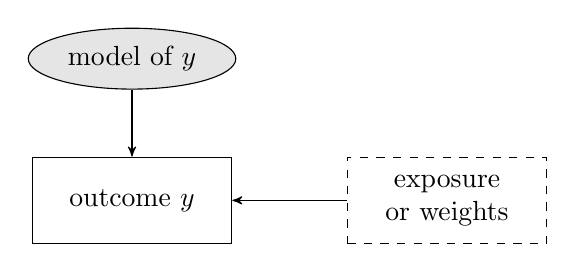
\begin{tikzpicture}
\tikzset{
   node distance = 3cm, >=stealth',
   array/.style = {rectangle, draw, minimum width = 2.3cm, minimum height = 1.1cm, text width = 2.3cm, align = center},
   model/.style = {ellipse, draw, fill = black!10, node distance = 1.8cm, minimum width = 2cm} 
}
  \node [array] (y) [] {outcome $y$};
  \node [array] (ew) [right of = y, dashed, xshift = 1cm] {exposure or weights}
        edge [->] (y);

  \node[model] (model_y) [above of = y] {model of $y$}
        edge [->] (y);

\end{tikzpicture}

\end{document}